% -----------------------------------------------------------------
%		 				 Dynamic Models
% -----------------------------------------------------------------
\begin{tcolorbox}[colback=green!5!white,colframe=green!75!black,title=Dynamic Models]
\textbf{Linear Time Invariant (LTI) Systems}\\
with A, B, C, D are matrices
\begin{equation*}
\dot { x } =Ax+Bu \quad y=Cx+Du 
\end{equation*}
\begin{equation*}
G(s)=C{ (sI-A) }^{ -1 }B+D
\end{equation*}

LTI sytems as Input-Output Models
\begin{equation*}
G(S)\, =\, \frac { b_0 + b_1s+...+b_ns^n }{ a_0+a_1s+...+a_{n-1}s^{n-1}+s^n } 
\end{equation*}

\textbf{Different Models}\\
\textbf{Deterministic Model:} \(y(k)=M(k;U,{ x }_{ init },p)\) \\
\textbf{Model with measurement Noise:} \\ \(y(k)=M(k;U,{ x }_{ init },p)+\varepsilon(k)\) \\
\textbf{Model with Input and Output Errors:} \\ \( \quad y(k)=M(k;U+{\varepsilon  }_{ N }^{ u },{ x }_{ init },p)+{ { \varepsilon }^{ y } }(k)\)


Pure Output Error (OE) Minimization
\begin{equation*}
\theta _{ ML } \, =\, arg\, \underset { \theta  }{ min } \, \sum _{ k=1 }^{ N }{ (y(k)-M(k;U,\, x_{ init }\, ,\, p)\, )^{ 2 } }
\end{equation*}

Output Error Minimization for FIR Models
\begin{equation*}
y(k) \, = \, (u(k),\, u(k-1),\, ...,\, u(k-n_{n_b})) \, \cdot \, \theta \, + \, \varepsilon(k)
\end{equation*}

\begin{equation*}
\underset { \theta  }{ min } \sum _{ k=n_{ b }+1 }^{ N }{ (\quad y(k)\, -\, (u(k),\, u(k-1),\, ...,\, u(k-n_{ n_{ b } }))\, \cdot \, \theta \quad )^{ 2 } } 
\end{equation*}


\begin{figure}[H]
	\centering
  	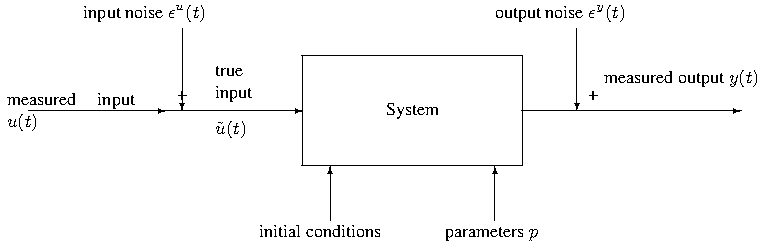
\includegraphics[width=\linewidth]{./model.pdf}
	\label{model}
\end{figure}
Models with Input and Output Errors
\begin{equation*}
arg \, \underset { \theta  }{ min } \, \sum _{ k-1 }^{ N }{ \frac { 1 }{ { \sigma  }_{ y }^{ 2 } }  } { (y(k)-M(k;U+{ \epsilon  }_{ N }^{ u },{ x }_{ init },p)) }^{ 2 }+\frac { 1 }{ { \sigma  }_{ u }^{ 2 } } { ({ \epsilon  }_{ u }(k)) }^{ 2 }
\end{equation*}


\begin{equation*}
arg \, \underset { \theta  }{ min } \, \sum _{ k-1 }^{ N }{ \frac { 1 }{ { \sigma  }_{ y }^{ 2 } }  } { (y(k)-M(k;\tilde { U } ,{ x }_{ init },p)) }^{ 2 }+\frac { 1 }{ { \sigma  }_{ u }^{ 2 } } { (u(k)-\tilde{ u }(k) ) }^{ 2 }
\end{equation*}
\end{tcolorbox}